\section{Abstract}
In this computer based test we are asked to perform linear regression by least squares on a given data set. The dataset analysed is the Olympic men's running time (100m and 400m) for a given range of years. 

In Task 1 we determine which polynomial function is the best fit for the 400m data. A common validation method is used to ensure the model is competent. In Task 2 we determine the best value of the regularisation factor, $\lambda$, for the polynomial functions of order 1 and 4.

In short, the results of Task 1 illustrate a polynomial function with order 2 best fits the Olympics men's 400m data. In Task 2, the results show a regularisation factor, $\lambda$, with value 0, gives the best predictive performance for both polynomial functions on the Olympic men's 100m data.

The analysis was performed in Matlab, and the code listings can be found in Appendices A and B.

\section{Task 1}{\label{s1}
	
\subsection{Introduction}\label{Int}
In Task 1, we are asked to analyse the Olympics men's 400m data. We must find the polynomial function of order \textbf{n} which best fits this data, where \textbf{n} is 1 to 4, and use 10-fold cross-validation to choose the "best" value of \textbf{n}. Refer to Appendix A for the Matlab code used for analysis.

To compute the average cross validation loss, data (attributes and labels) are separated into 10 partitions (i.e. 10-fold), where 1 partition is reserved for testing the model. The 9 remaining partitions are used to learn the model with parameters, $w_{n}$. This models can use the attributes of the test partition to predict the labels, in this case the time ran for the men's 400m. The predicted values can then be compared to the actual values (labels)  from the test partition. The cross validation (CV) loss is calculated by taking the mean squared difference ($msd$) of these two values. This is then repeated 9 more times by rotating the test partition through. The average of these 10 $msd$ values is calculated and then plotted against the order to find the minimum value.
\subsection{Results}\label{CVcons}
From Figure \ref{fig:CVT4} and Table \ref{t:ModLoss} it is shown that a polynomial function with order 4 is the best fit. However, in order to determine the "best" order, it must be given a concrete meaning for this task. "Best" is considered to be the minimum mean squared loss, where loss is the difference between predicted and observed labels. Ideally, both cross-validation (CV) and training loss are considered but that is not always the case. So, three cases are defined as the following.

\begin{enumerate}
	\item Only CV loss is considered
	\item Only Train loss is considered
	\item Both CV and Train loss are considered
\end{enumerate}

\begin{figure}[h]
	\centering
	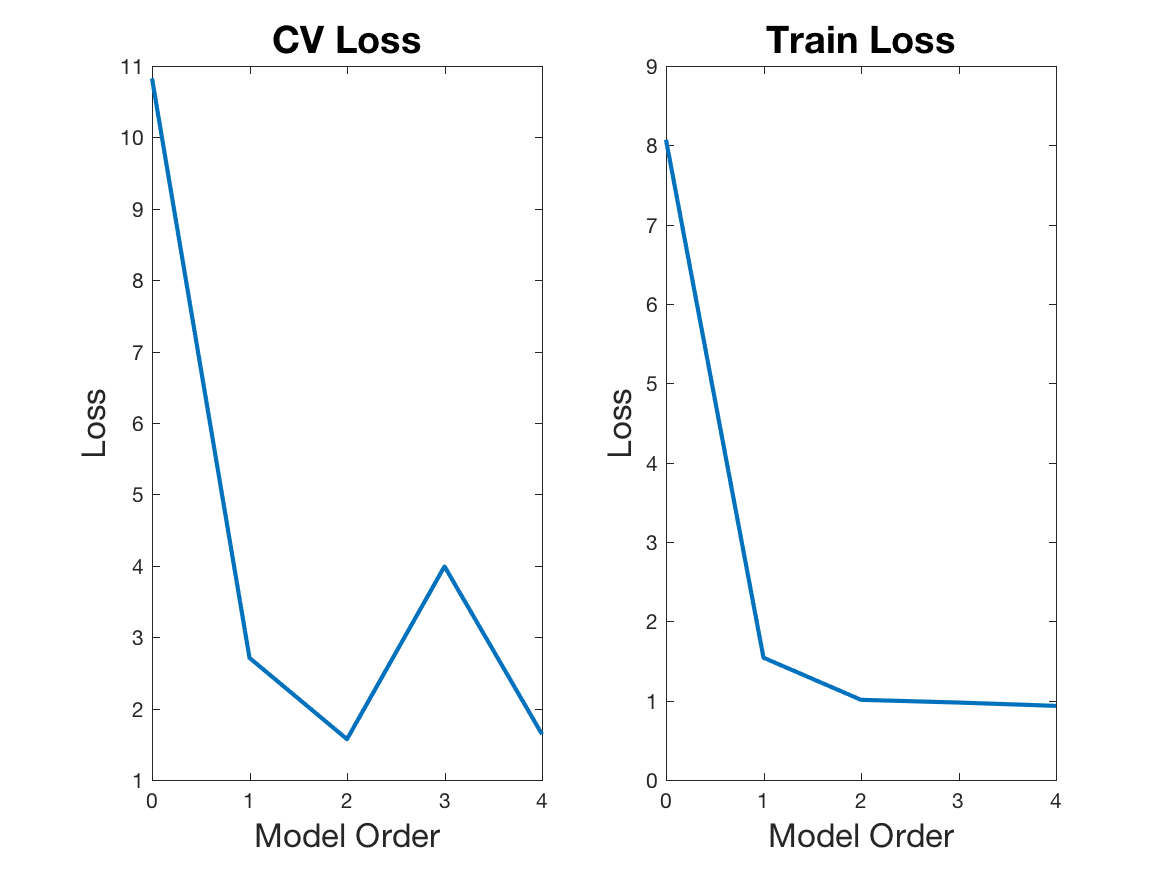
\includegraphics[width=0.8\linewidth]{images/CVLossANDTrainLoss4}
	\caption{Comparison of the CV and Train loss for polynomial models of order \textbf{n}, where \textbf{n} = 0 to 4.}
	\label{fig:CVT4}
\end{figure}

\begin{table}[h]
	\centering
	\caption{Summary of Model Losses}
	\label{t:ModLoss}
	\begin{tabular}{rrrr}
		\hline
		\textbf{Order} & \textbf{CV Loss} & \textbf{Train Loss} & \textbf{Average Squared Loss} \\ \hline
		0 & 10.83 & 8.07 & 178.61 \\
		1 & 2.71 & 1.54 & 9.03 \\
		2 & 1.57 & 1.01 & 3.33 \\
		3 & 3.99 & 0.98 & 12.35 \\
		4 & 1.64 & 0.93 & 3.30
	\end{tabular}
\end{table}

Consider item 1, Figure \ref{fig:CVT4} and Table \ref{t:ModLoss} show that a polynomial function with order 2 is the best fit. It is visualised clearly on Figure \ref{fig:CVT4} as the minimum point on the line. Looking at Table \ref{t:ModLoss}, a minimum value of 1.57 also corresponds with order 2.

Consider item 2, Figure \ref{fig:CVT4} and Table \ref{t:ModLoss} show that a polynomial function with order 4 is the best fit. Figure \ref{fig:CVT4} shows a downward trend to the right, indicating that an order of 4 is indeed the best fit. Looking at Table \ref{t:ModLoss}, the minimum value, 3.30, also corresponds with an order of 4.

Consider item 3, Figure \ref{fig:CVT4} and Table \ref{t:ModLoss} show that a polynomial function with order 4 is the best fit. It is difficult to see this via the visualisation of Figure \ref{fig:CVT4}. However, looking at Table \ref{t:ModLoss}, the average squared loss (of CV and Train loss) is lowest when order equals 4. 

\begin{figure}[h!] 
	\centering
	\begin{subfigure}[b]{0.4\textwidth}
		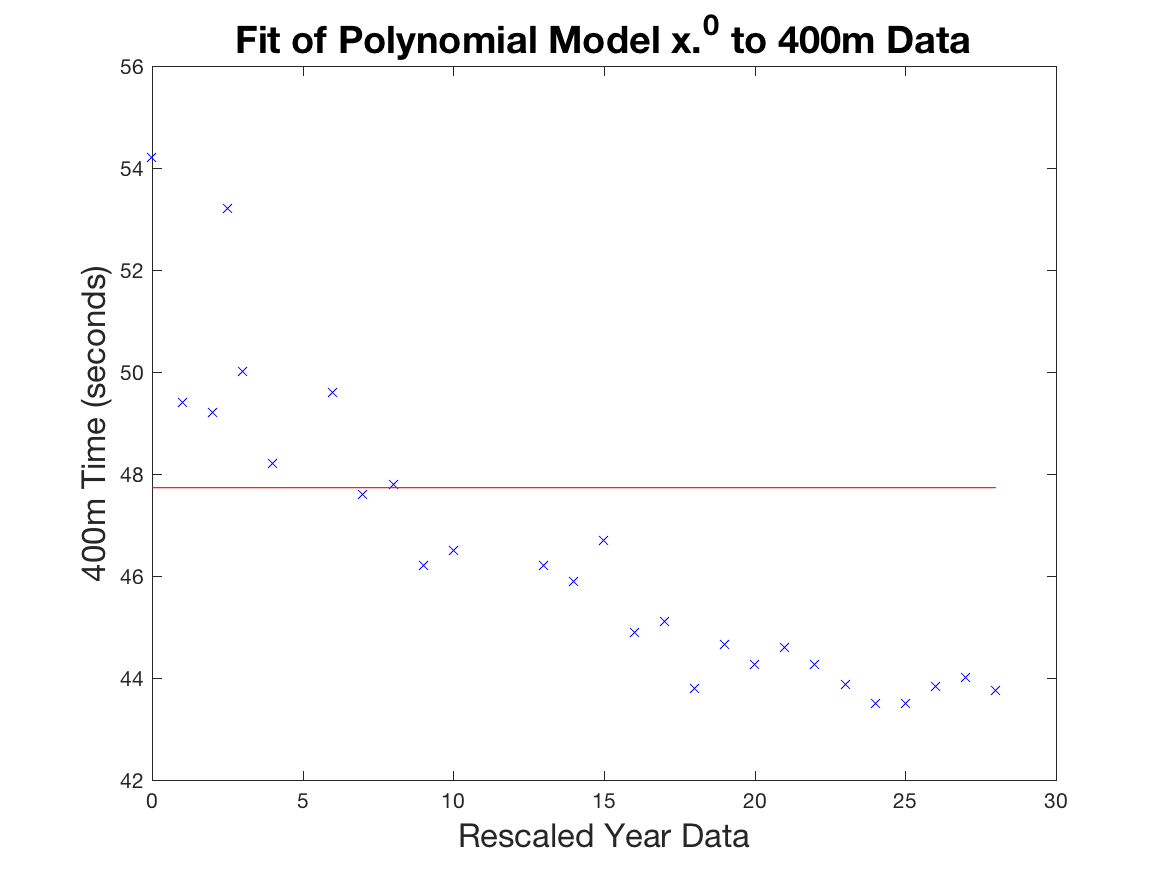
\includegraphics[width=\textwidth]{model0.png}
		\caption{Polynomial model with order \textbf{n} = 0}
		\label{fig:model0}
	\end{subfigure}
	\begin{subfigure}[b]{0.4\textwidth}
		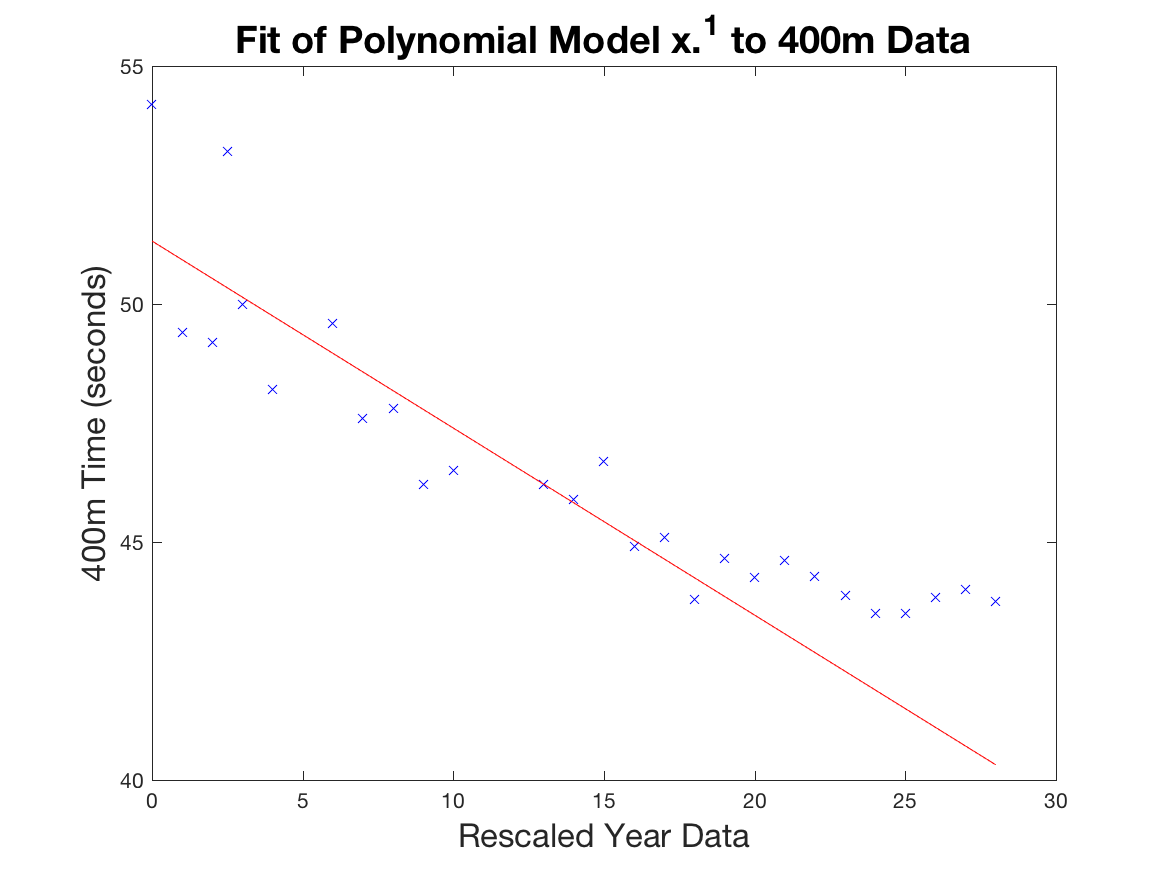
\includegraphics[width=\textwidth]{model1.png}
		\caption{Polynomial model with order \textbf{n} = 1}
		\label{fig:model1}
	\end{subfigure}
	\begin{subfigure}[b]{0.4\textwidth}
		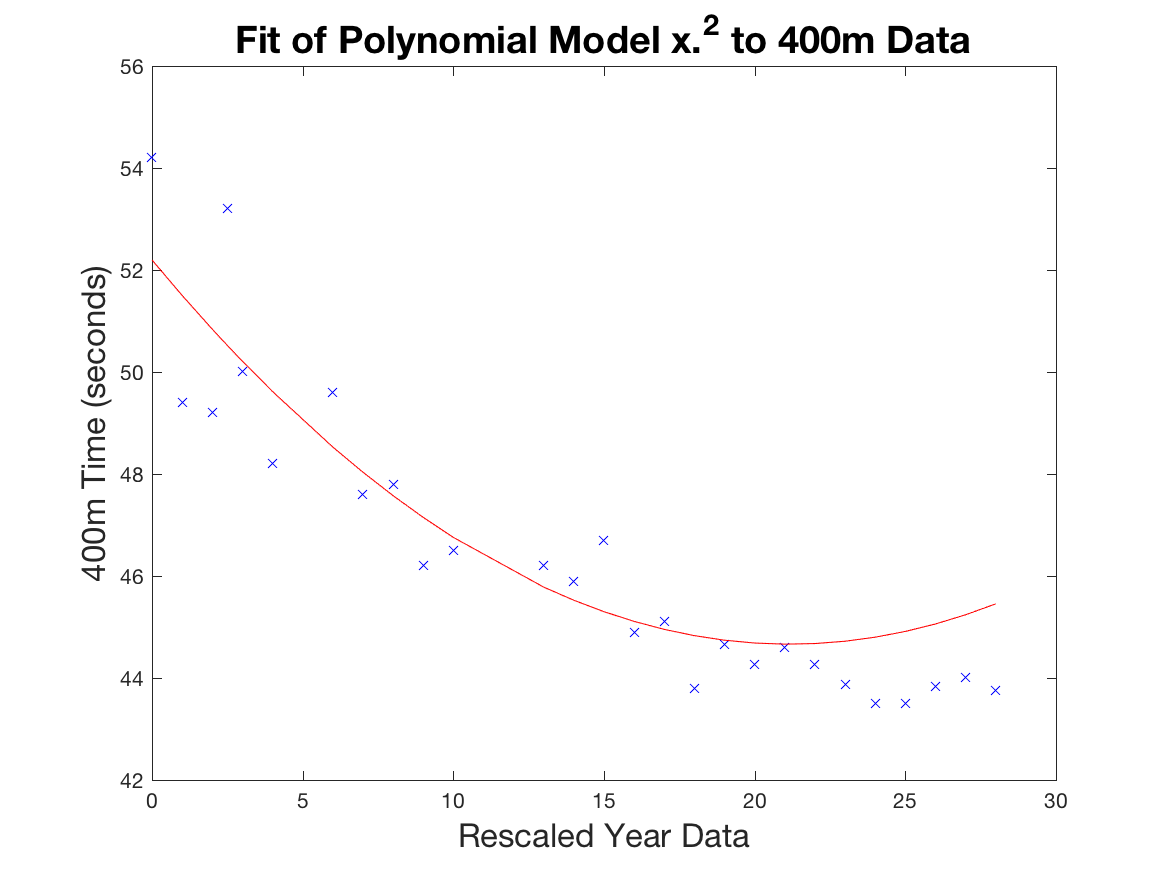
\includegraphics[width=\textwidth]{model2.png}
		\caption{Polynomial model with order \textbf{n} = 2}
		\label{fig:model2}
	\end{subfigure}
	\begin{subfigure}[b]{0.4\textwidth}
		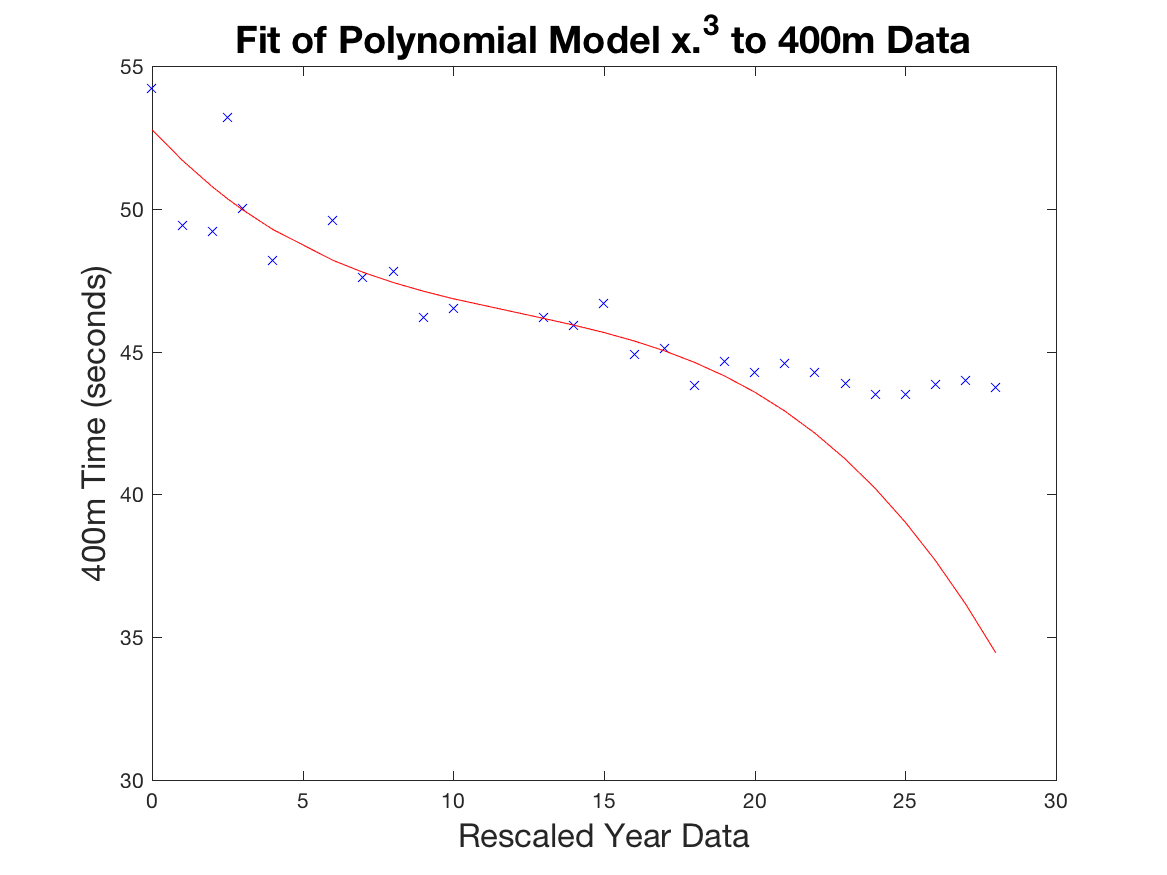
\includegraphics[width=\textwidth]{model3.png}
		\caption{Polynomial model with order \textbf{n} = 3}
		\label{fig:model3}
	\end{subfigure}
	\begin{subfigure}[b]{0.4\textwidth}
		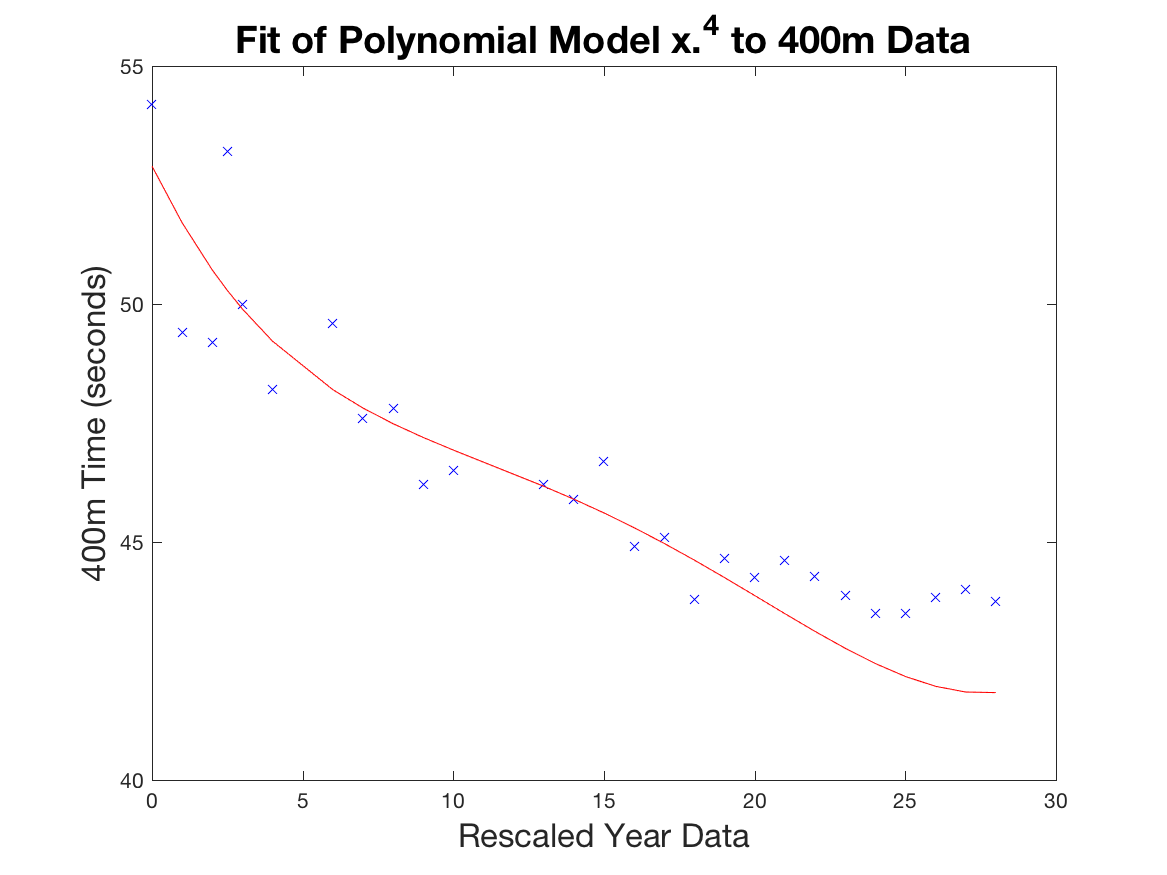
\includegraphics[width=\textwidth]{model4.png}
		\caption{Polynomial model with order \textbf{n} = 4}
		\label{fig:model4}
	\end{subfigure}
	\caption{The original Olympic men's 400m data (blue crosses) with the polynomial models (red) overlaid.}
	\label{men400-1}
\end{figure}

Figure \ref{fig:model2} shows how well each of the models fit the data. Interestingly, Figure \ref{fig:model4}, shows an order of 4 provides an accurate model and more realistic future predictions than an order of 2. In comparison, an order of 2 shows that future predictions would increase in time at an increasing rate. This is highly unlikely given the downward trend of the data.

The remaining models in Figure \ref{men400-1} clearly do not model the data well, where orders 1 and 3 show that a time of 0 will be achieved soon. This is not humanly possibly so the models can be discarded. 

\subsection{Conclusion}
The problem for Task 1 is to find the "best model based on average cross-validation loss." This only considers point 1 from before, therefore, a polynomial function with order 2 best fits the model based on average cross-validation loss.

\subsection{Further Comments}
Further investigation found if the data was not standardised, a systematic error is produced in the model for orders greater than or equal 4. Figure \ref{men400-1noSt} illustrates an order of 3 produces no error, but an order of 4 does. Reviewing literature showed this systematic error is common when dealing with high order polynomial function\cite{WhenIsIt}.Therefore, it is good practice to standardise data when the regression model contains polynomial terms.

\begin{figure}[h!] 
	\centering
	\begin{subfigure}[b]{0.4\textwidth}
		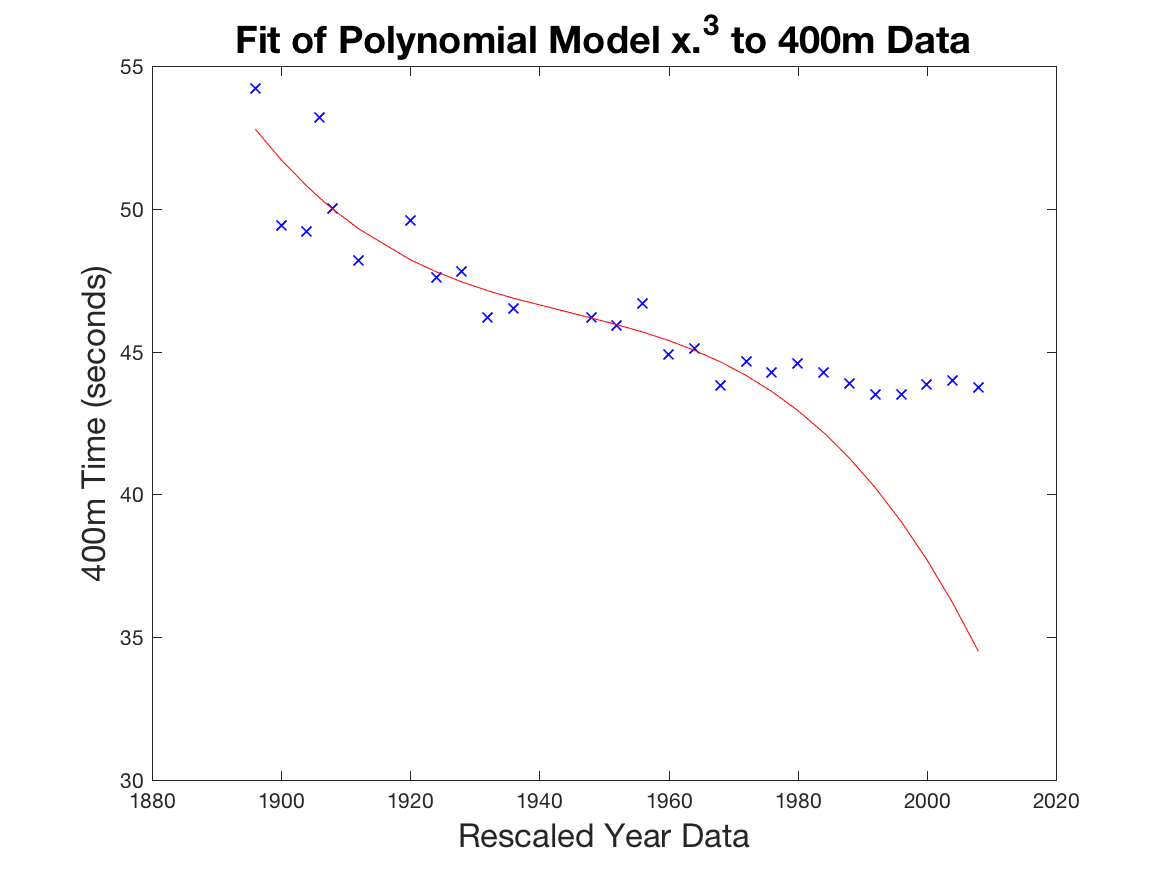
\includegraphics[width=\textwidth]{modelNotReg3.png}
		\caption{Polynomial model with order \textbf{n} = 3}
		\label{fig:modelNoReg0}
	\end{subfigure}
	\begin{subfigure}[b]{0.4\textwidth}
		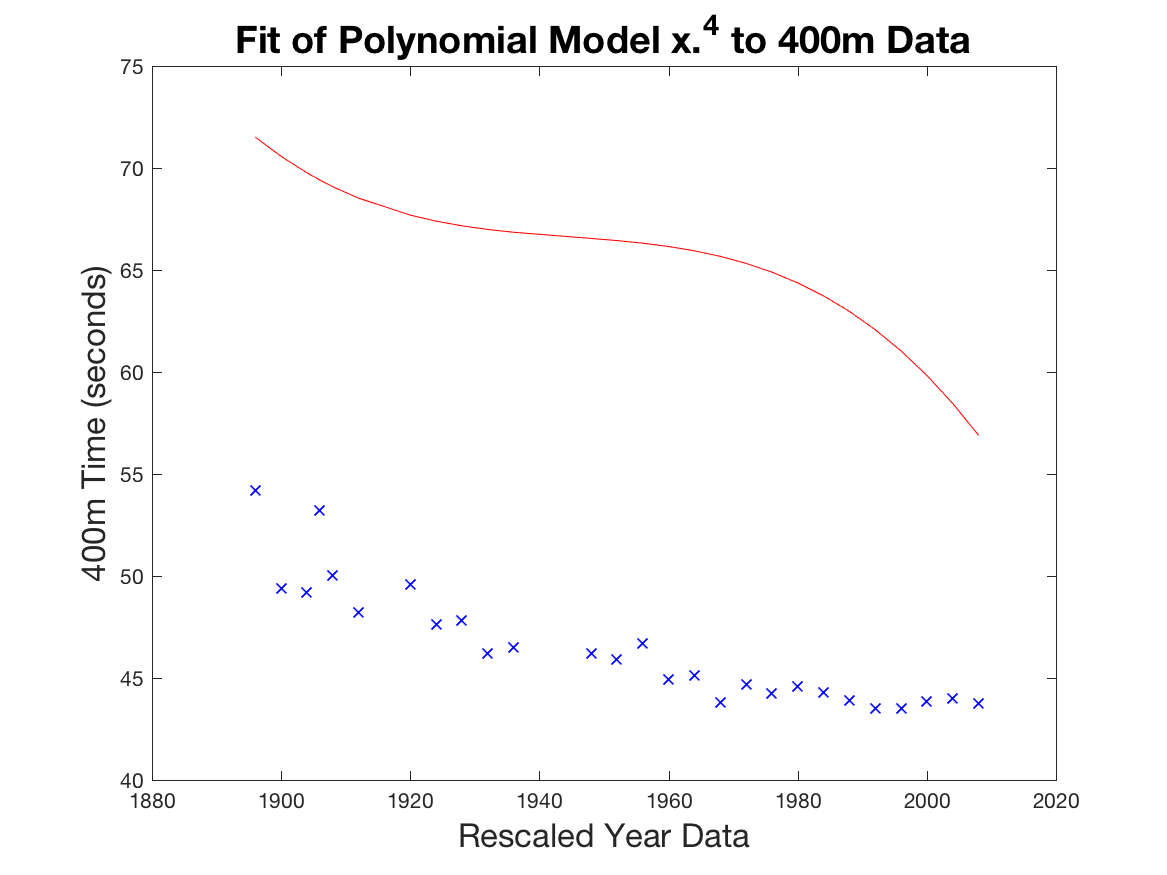
\includegraphics[width=\textwidth]{modelNotReg4.png}
		\caption{Polynomial model with order \textbf{n} = 4}
		\label{fig:modelNoReg1}
	\end{subfigure}
	\caption{The original Olympic men's 400m data (blue crosses) with the polynomial models (red) overlaid without data standardisation.}
	\label{men400-1noSt}
\end{figure}

Another point worth mentioning is the effect of permuting (randomising) the attributes. For this small dataset the permutations caused some instability in the model and different results were obtained as can be seen in Figure \ref{men400CVRandSt}. The results of the permuted data agree with the results from before.

\begin{figure}[h!] 
	\centering
	\begin{subfigure}[b]{0.35\textwidth}
		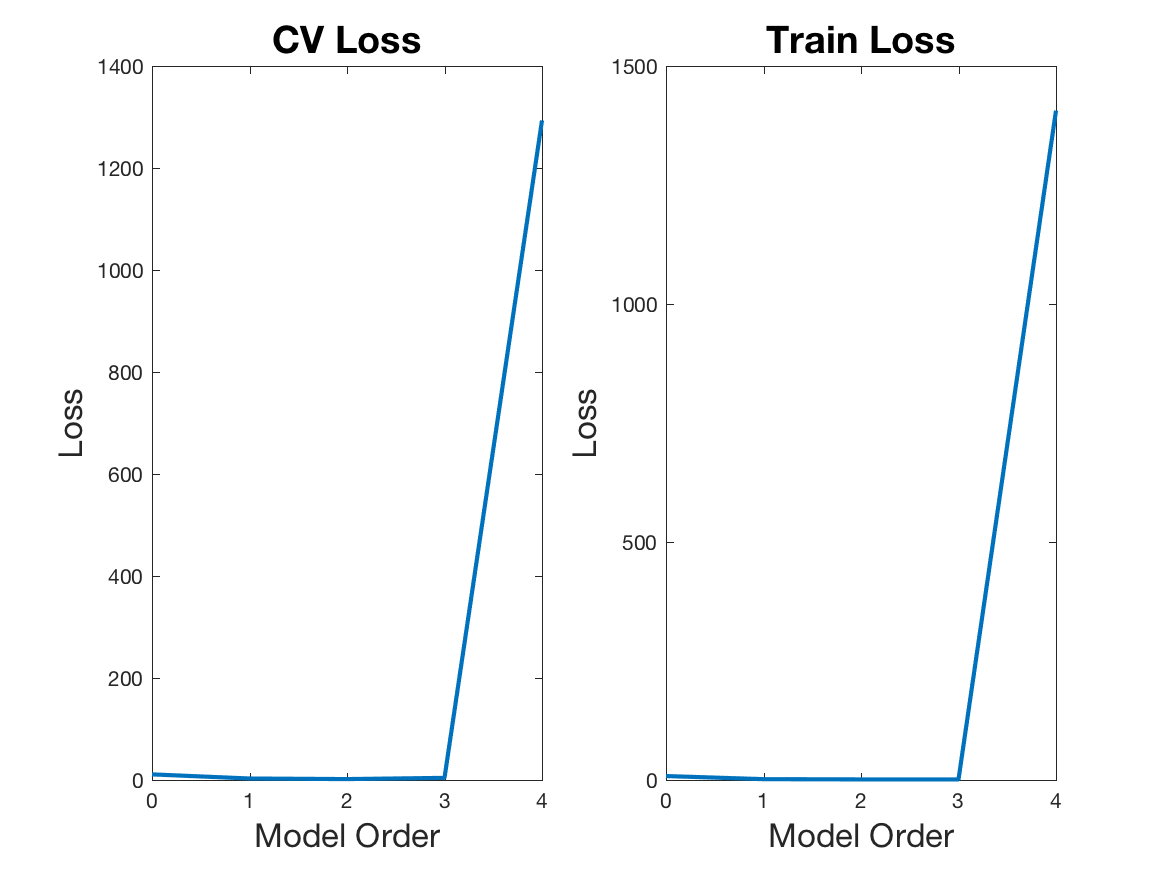
\includegraphics[width=\textwidth]{CVLossANDTrainLossNotReg4.png}
		\caption{CV and Train loss when the data is not standardised}
		\label{fig:modelNoRegCV}
	\end{subfigure}
	\begin{subfigure}[b]{0.35\textwidth}
		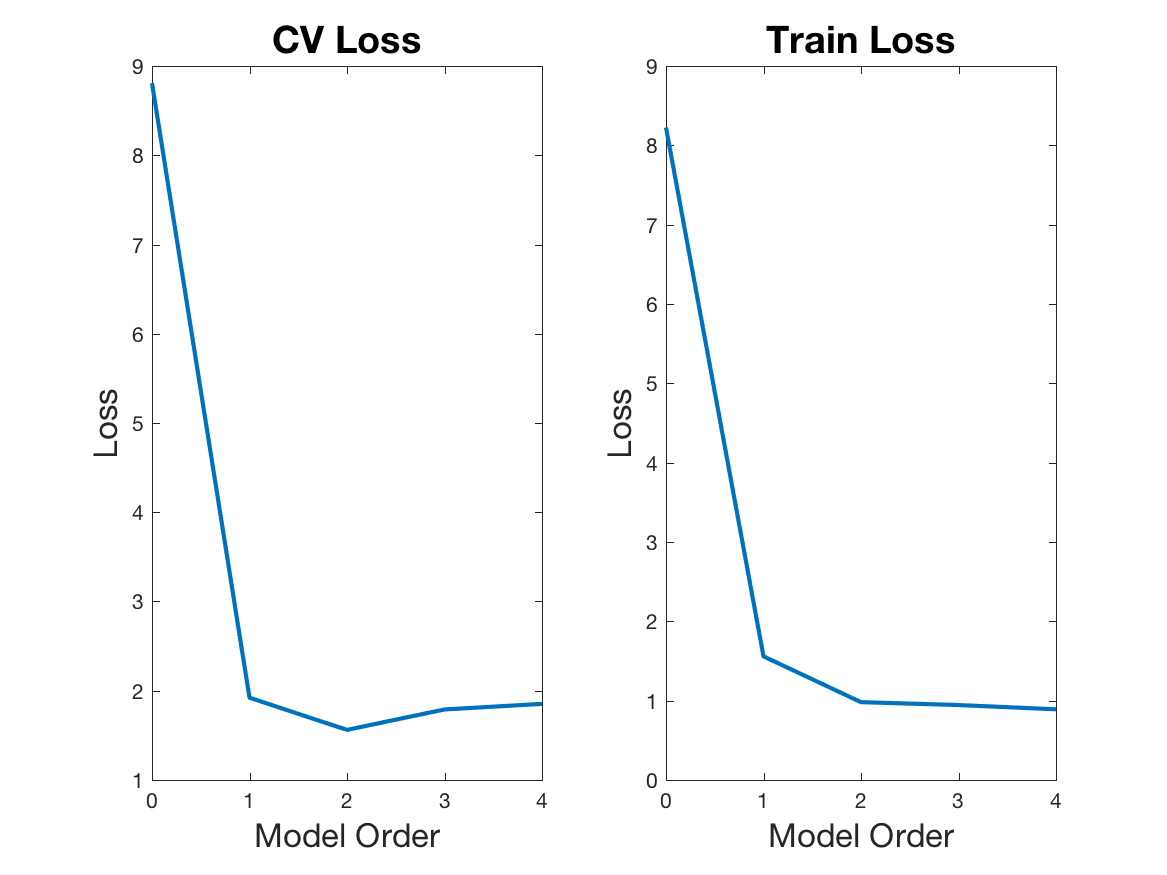
\includegraphics[width=\textwidth]{CVLossANDTrainLossRand.png}
		\caption{CV and train loss with permuted data}
		\label{fig:modelRand}
	\end{subfigure}
	\caption{Comparision of the CV and Train Loss when it is not standardised (\ref{fig:modelNoRegCV}) and data is permuted (\ref{fig:modelRand}).}
	\label{men400CVRandSt}
\end{figure}

\section{Task 2}
\subsection{Introduction}
In task 2 we are given the task to find the value of $\lambda$ that gives the 'best' predictive performance on the Olympic men's 100m data using 5-fold cross-validation. In this task, "best" is also defined the same as in \ref{s1}. Refer to Appendix B for the Matlab code used for analysis.

Task 2 uses the same method as Task 1, however, an additional parameter, $\lambda$, is introduced. The calculation for the CV loss essentially remains the same as described in \ref{int}, except now higher order models (complexity) are penalised by the $\lambda$ value.

\subsection{Results}
Figure \ref{fig:LambdaLoss} shows that the best value for $\lambda$ is 0 for this dataset. However, there is an interesting trend for both orders, where it increases until some value and then there is a local minimum. If this is a common trend, and 0 is not always the minimum, this local minimum could be a desired value to minimise loss. 


\begin{figure}[h!]
	\centering
	\begin{subfigure}[b]{0.45\textwidth}
		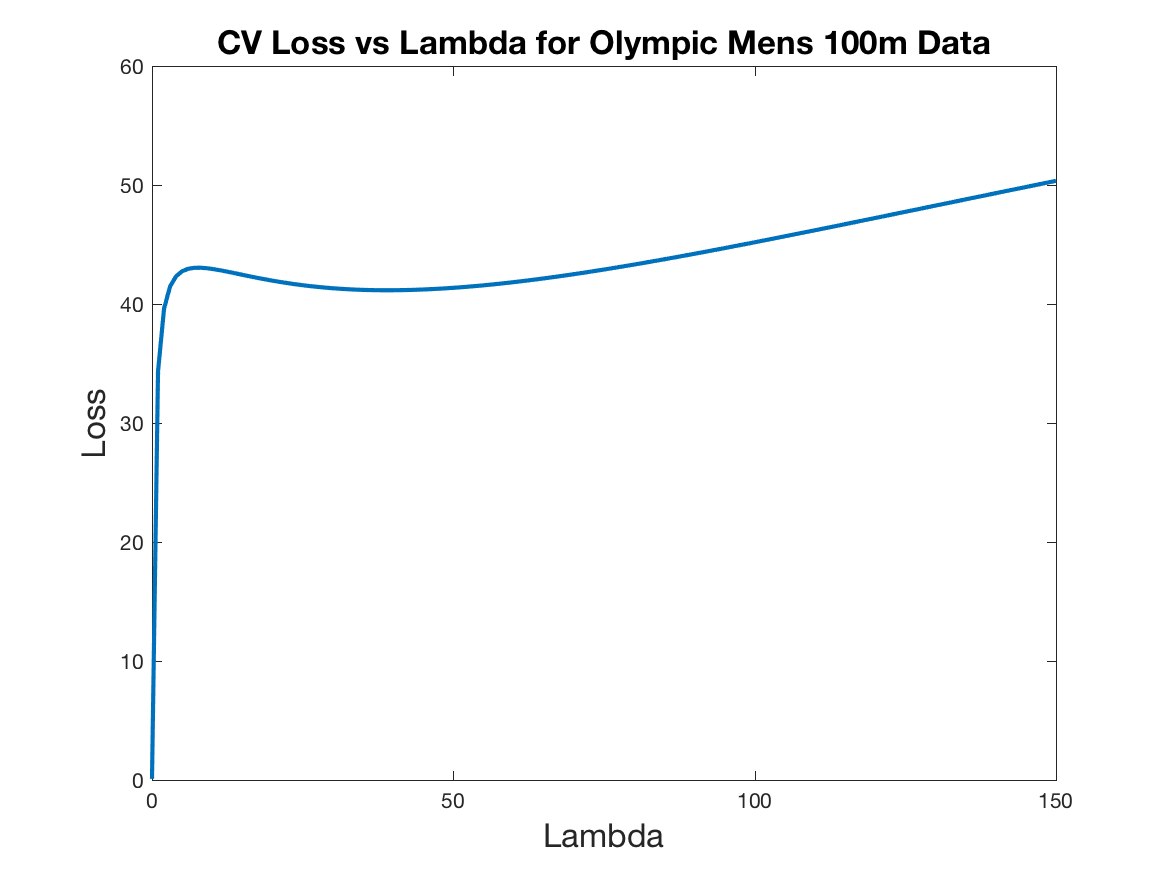
\includegraphics[width=\textwidth]{CVLossvsLambda1.png}
		\caption{Loss of varying lambda values for order 1}
		\label{fig:CVLL1}
	\end{subfigure}
	\begin{subfigure}[b]{0.45\textwidth}
		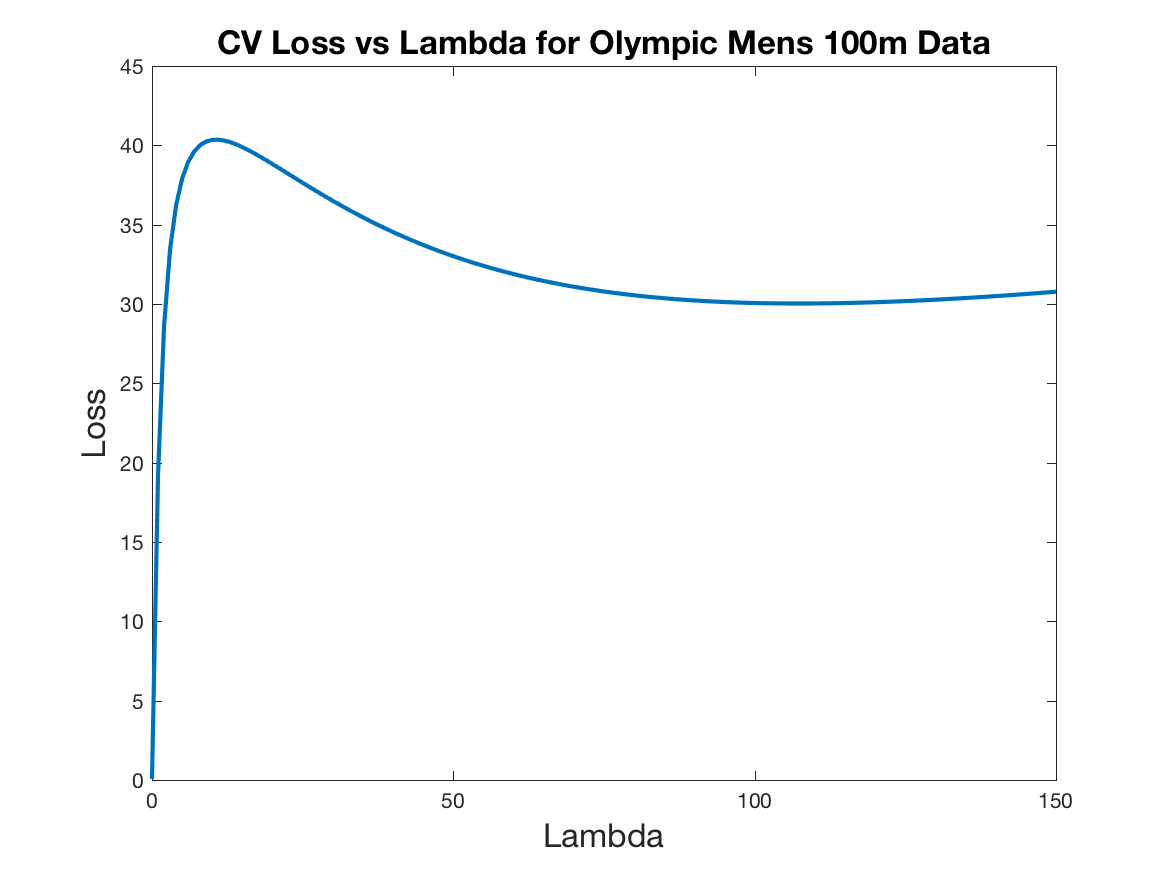
\includegraphics[width=\textwidth]{CVLossvsLambda4.png}
		\caption{Loss of varying lambda values for order 4}
		\label{fig:CVLL4}
	\end{subfigure}
	\caption{The loss vs lambda values for polynomial models with order 1, and 4.}
	\label{fig:LambdaLoss}
\end{figure}

Although a large range of $\lambda$ is plotted on \ref{fig:LambdaLoss} , is should be noted that the value is very sensitive. This is evidenced by Figures \ref{fig:lambda1} and \ref{fig:lambda2}, where the  $\lambda$ value only varies from 0 to 0.3. The figures indicate there is a model loss even for a $\lambda$ value of 0.1.

\begin{figure}[h!] 
	\centering
	\begin{subfigure}[b]{0.4\textwidth}
		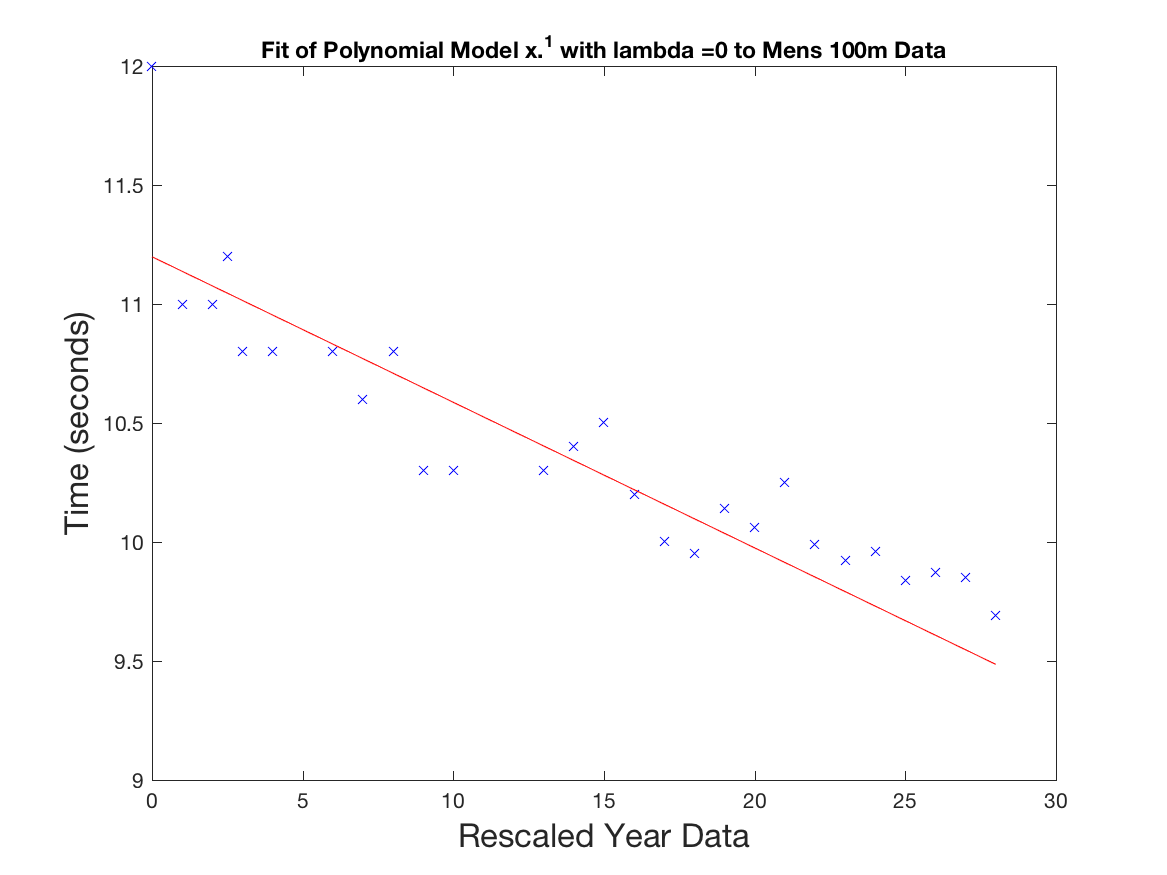
\includegraphics[width=\textwidth]{LambdaModel0_1.png}
		\caption{Lambda = 0}
		\label{fig:model0}
	\end{subfigure}
	\begin{subfigure}[b]{0.4\textwidth}
		\includegraphics[width=\textwidth]{{LambdaModel0.1_1}.png}
		\caption{Lambda = 0.1}
		\label{fig:model1}
	\end{subfigure}
	\quad
	\begin{subfigure}[b]{0.4\textwidth}
		\includegraphics[width=\textwidth]{{LambdaModel0.2_1}.png}
		\caption{Lambda = 0.2}
		\label{fig:model0}
	\end{subfigure}
	\begin{subfigure}[b]{0.4\textwidth}
		\includegraphics[width=\textwidth]{{LambdaModel0.3_1}.png}
		\caption{Lambda = 0.3}
		\label{fig:model1}
	\end{subfigure}
	\caption{Polynomial model with order 1 and varying lambda values.}
	\label{fig:lambda1}
\end{figure}

\begin{figure}[h!]
	\centering
	\begin{subfigure}[b]{0.4\textwidth}
		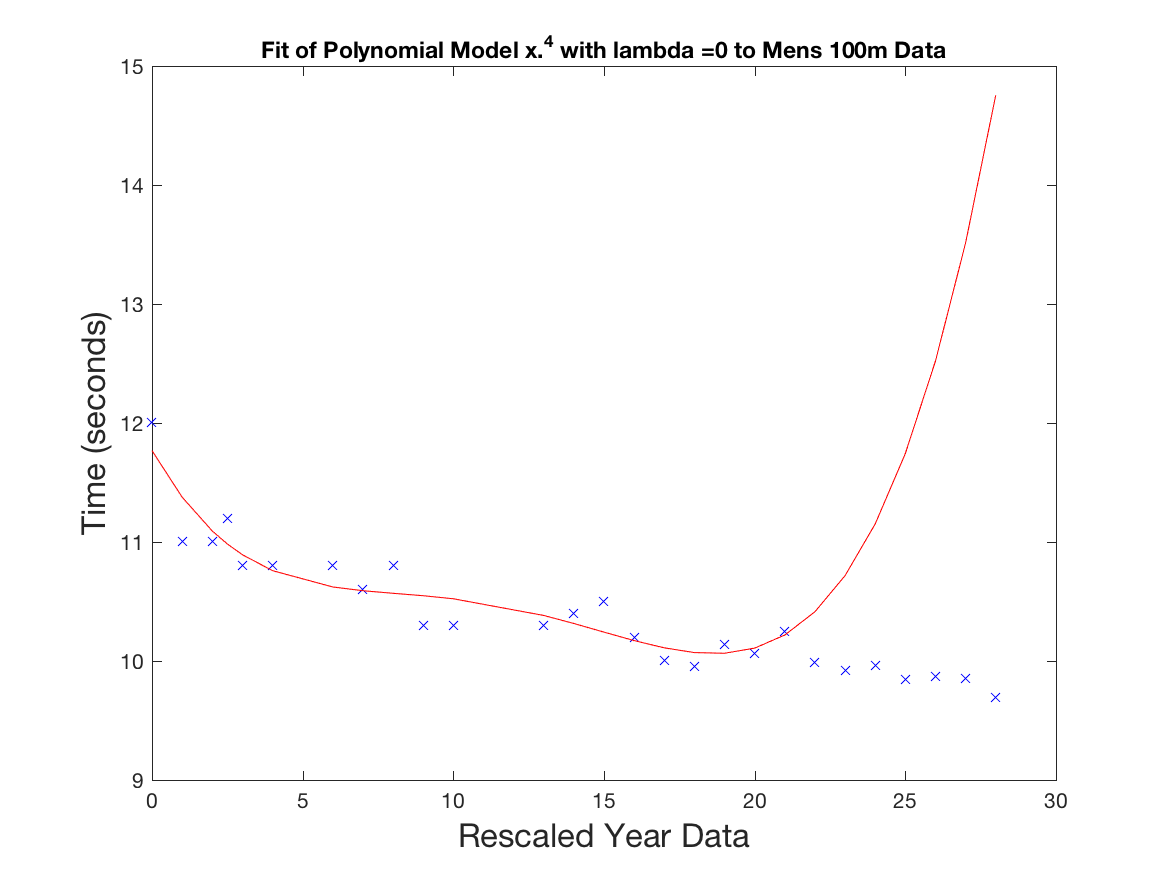
\includegraphics[width=\textwidth]{LambdaModel0_4.png}
		\caption{Lambda = 0}
		\label{fig:model0}
	\end{subfigure}
	\begin{subfigure}[b]{0.4\textwidth}
		\includegraphics[width=\textwidth]{{LambdaModel0.1_4}.png}
		\caption{Lambda = 0.1}
		\label{fig:model1}
	\end{subfigure}
	\quad
	\begin{subfigure}[b]{0.4\textwidth}
		\includegraphics[width=\textwidth]{{LambdaModel0.2_4}.png}
		\caption{Lambda = 0.2}
		\label{fig:model0}
	\end{subfigure}
	\begin{subfigure}[b]{0.4\textwidth}
		\includegraphics[width=\textwidth]{{LambdaModel0.3_4}.png}
		\caption{Lambda = 0.3}
		\label{fig:model1}
	\end{subfigure}
	\caption{Polynomial model with order 4 and varying lambda values.}
	\label{fig:lambda2}
\end{figure}

\subsection{Conclusion}
The problem for Task 2 is "using 5-fold cross-validation, find the value of $\lambda$ that gives the “best” predictive performance on the Olympic men’s 100m for 1st and 4th order polynomials." Predictive performance only considers CV loss, as described in point 1 in Section \ref{CVcons}. Therefore, referring to Figure \ref{fig:LambdaLoss}, it is clear $\lambda$ with value 0, gives the best predictive performance.  

\subsection{Further Comments}
Further investigation showed that permuting the data also introduced instability for this small dataset as shown in Figure \ref{fig:LambdaLossR}. Interestingly, this removes the local minimum found in \ref{fig:LambdaLoss}, which may disprove the hypothesis that a $\lambda$ value for a local minima is desired. 

The results of the permuted data supports the hypothesis that a $\lambda$ value of 0 gives the best predictive performance for the Olympics men's 100m data.

\begin{figure}[h] %example of figure with picture 'h' tells latex to place it 'around' here
	\centering
	\begin{subfigure}[b]{0.45\textwidth}
		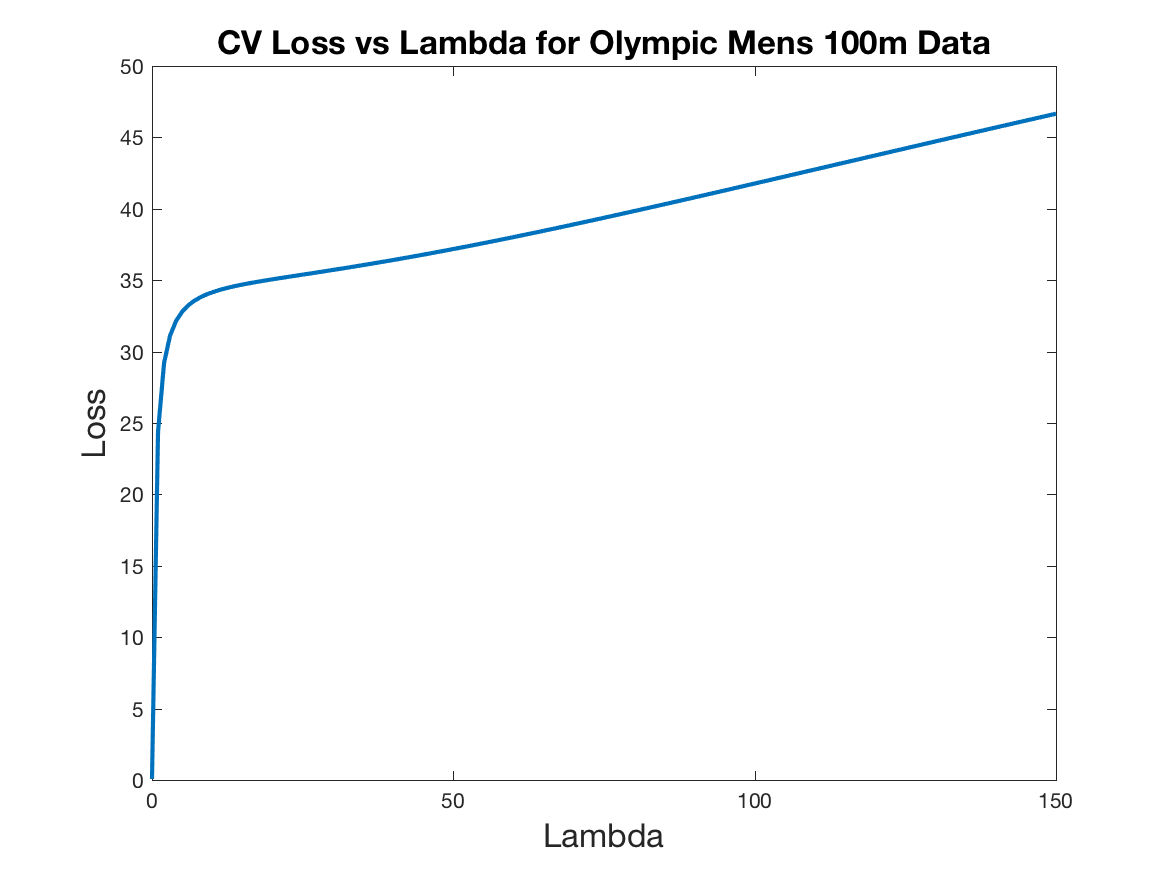
\includegraphics[width=\textwidth]{CVLossvsLambdaRand1.png}
		\caption{Loss of varying lambda values for order 1}
		\label{fig:CVLL1R}
	\end{subfigure}
	\begin{subfigure}[b]{0.45\textwidth}
		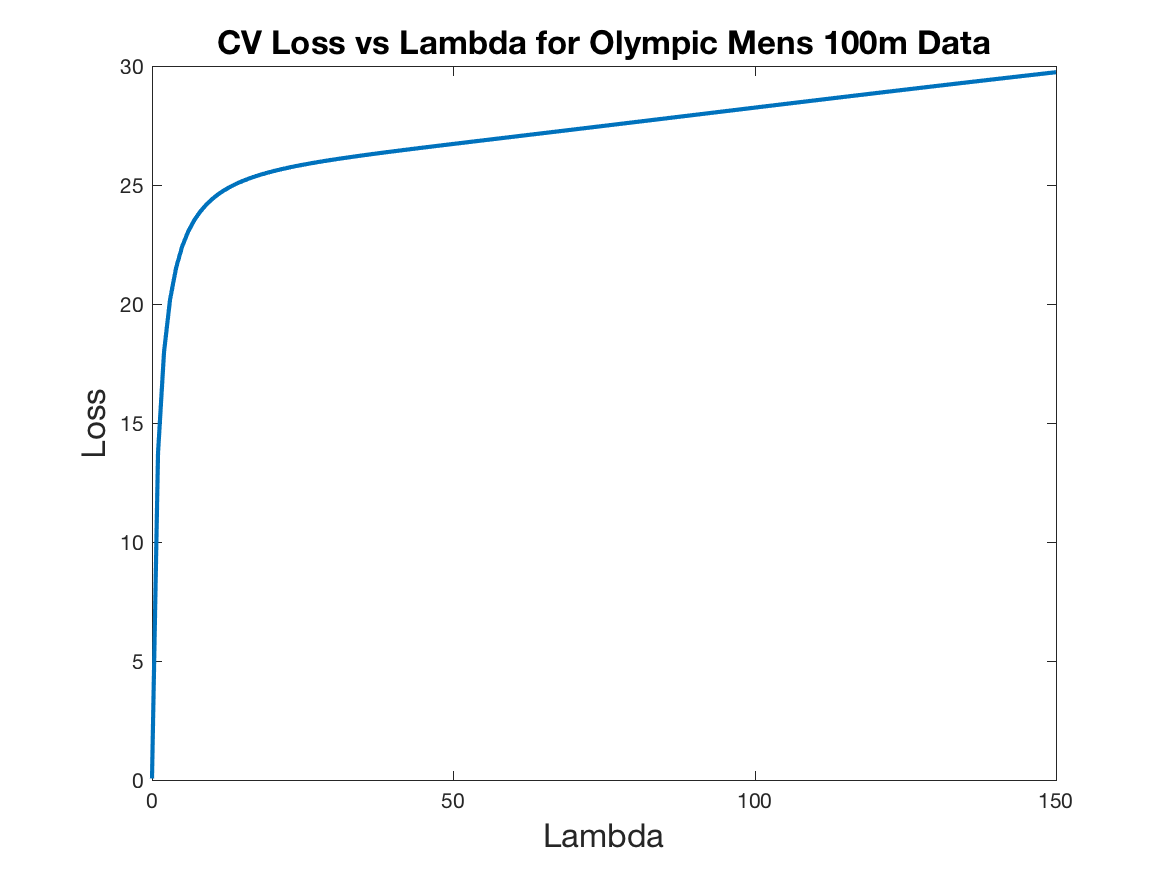
\includegraphics[width=\textwidth]{CVLossvsLambdaRand4.png}
		\caption{Loss of varying lambda values for order 4}
		\label{fig:CVLL4R}
	\end{subfigure}
	\caption{The loss vs lambda values for polynomial models with order 1, and 4 with permuted data.}
	\label{fig:LambdaLossR}
\end{figure}
